\documentclass[10pt]{beamer}

\usepackage[T1]{fontenc}

\usetheme{metropolis}

\usepackage{graphicx}
\graphicspath{{images/}}
\usepackage{amsmath, amssymb, amsthm}
\usepackage{mathtools}
\usepackage{bm}
\usepackage{booktabs}
\usepackage{caption}
\usepackage{array}
\usepackage{tikz}
\usetikzlibrary{positioning, arrows.meta, calc}
\usepackage{listings}
\usepackage{xcolor}
\usepackage[numbers,square]{natbib}
\usepackage[most]{tcolorbox}
\usepackage{tabularx}
\definecolor{codebg}{RGB}{245,245,245}
\definecolor{codeframe}{RGB}{180,180,180}
\definecolor{boxbg}{RGB}{235,245,255}
\definecolor{boxframe}{RGB}{70,130,180}
\definecolor{ctrl}{HTML}{EB6834}   % P.ORANGE: the control, as in the figures

\lstdefinestyle{pytorch}{
  language=Python,
  basicstyle=\ttfamily\scriptsize,
  keywordstyle=\color{blue!70!black}\bfseries,
  stringstyle=\color{green!50!black},
  commentstyle=\color{gray}\itshape,
  showstringspaces=false,
  breaklines=true,
  columns=fullflexible,
  backgroundcolor=\color{codebg},
  frame=single,
  rulecolor=\color{codeframe},
  framesep=4pt,
  xleftmargin=4pt,
  xrightmargin=4pt,
}
\lstset{style=pytorch}

\title{Universal Approximation and Optimization}
\subtitle{Mathematical Foundations of Control and Machine Learning}
\author{Enrique Zuazua, Daniel L\'opez Montero}
\date{Winter 2026}
\institute{FAU Erlangen-N\"urnberg}

% --- Math shortcuts --------------------------------------------------------
\newcommand{\R}{\mathbb{R}}
\newcommand{\N}{\mathbb{N}}
\newcommand{\E}{\mathbb{E}}
\newcommand{\Gram}{\mathcal{G}}
\newcommand{\ctrl}[1]{\textcolor{ctrl}{#1}}
\DeclareMathOperator{\Range}{Range}
\DeclareMathOperator*{\argmin}{arg\,min}

% --- A box for definitions and theorems ------------------------------------
\newtcolorbox{mathbox}[2][]{
  colback=boxbg, colframe=boxframe, boxrule=0.2pt, arc=2pt,
  left=4pt, right=4pt, top=2pt, bottom=2pt,
  title=\textbf{#2}, fonttitle=\small, coltitle=white, colbacktitle=boxframe,
  halign=left, #1}

% --- Notebook references for worked examples and exercises only ------------
\newcommand{\nbref}[1]{%
  \begin{tikzpicture}[remember picture, overlay]
    \node[anchor=south west, font=\scriptsize, text=black!55]
      at ([xshift=5mm, yshift=1.1mm] current page.south west) {Notebook #1};
  \end{tikzpicture}}

\setbeamerfont{standout}{size=\Large, series=\mdseries}
\setbeamertemplate{bibliography item}[text]
\renewcommand{\bibsection}{}

% --- Bibliography database -------------------------------------------------
% The entries live here so that the slides are one self-contained file.  Each
% compilation writes them to universal_approximation_and_optimization.bib for
% BibTeX: edit this block, not the generated .bib file.
\begin{filecontents}[overwrite]{universal_approximation_and_optimization.bib}
@article{weierstrass1885,
  author  = {Weierstrass, Karl},
  title   = {{\"U}ber die analytische {D}arstellbarkeit sogenannter willk{\"u}rlicher {F}unctionen einer reellen {V}er{\"a}nderlichen},
  journal = {Sitzungsberichte der K{\"o}niglich Preu{\ss}ischen Akademie der Wissenschaften zu Berlin},
  pages   = {633--639, 789--805},
  year    = {1885}
}

@article{wiener1932,
  author  = {Wiener, Norbert},
  title   = {Tauberian Theorems},
  journal = {Annals of Mathematics},
  volume  = {33},
  number  = {1},
  pages   = {1--100},
  year    = {1932},
  doi     = {10.2307/1968102}
}

@article{courant1943,
  author  = {Courant, Richard},
  title   = {Variational Methods for the Solution of Problems of Equilibrium and Vibrations},
  journal = {Bulletin of the American Mathematical Society},
  volume  = {49},
  pages   = {1--23},
  year    = {1943},
  doi     = {10.1090/S0002-9904-1943-07818-4}
}

@article{cybenko1989,
  author  = {Cybenko, George},
  title   = {Approximation by Superpositions of a Sigmoidal Function},
  journal = {Mathematics of Control, Signals, and Systems},
  volume  = {2},
  pages   = {303--314},
  year    = {1989},
  doi     = {10.1007/BF02551274}
}

@article{leshno1993,
  author  = {Leshno, Moshe and Lin, Vladimir Ya. and Pinkus, Allan and Schocken, Shimon},
  title   = {Multilayer Feedforward Networks with a Nonpolynomial Activation Function Can Approximate Any Function},
  journal = {Neural Networks},
  volume  = {6},
  number  = {6},
  pages   = {861--867},
  year    = {1993},
  doi     = {10.1016/S0893-6080(05)80131-5}
}

@book{nocedal2006,
  author    = {Nocedal, Jorge and Wright, Stephen J.},
  title     = {Numerical Optimization},
  edition   = {2},
  publisher = {Springer},
  address   = {New York},
  year      = {2006},
  doi       = {10.1007/978-0-387-40065-5}
}

@article{polyak1964,
  author  = {Polyak, Boris T.},
  title   = {Some Methods of Speeding up the Convergence of Iteration Methods},
  journal = {USSR Computational Mathematics and Mathematical Physics},
  volume  = {4},
  number  = {5},
  pages   = {1--17},
  year    = {1964},
  doi     = {10.1016/0041-5553(64)90137-5}
}

@article{nesterov1983,
  author  = {Nesterov, Yurii E.},
  title   = {A Method for Solving the Convex Programming Problem with Convergence Rate {$O(1/k^2)$}},
  journal = {Doklady Akademii Nauk SSSR},
  volume  = {269},
  number  = {3},
  pages   = {543--547},
  year    = {1983}
}

@misc{hinton2012,
  author       = {Hinton, Geoffrey},
  title        = {Neural Networks for Machine Learning, Lecture 6: Overview of Mini-Batch Gradient Descent},
  howpublished = {Coursera lecture slides},
  year         = {2012},
  url          = {https://www.cs.toronto.edu/~hinton/coursera/lecture6/lec6.pdf}
}

@inproceedings{kingma2015,
  author    = {Kingma, Diederik P. and Ba, Jimmy},
  title     = {Adam: A Method for Stochastic Optimization},
  booktitle = {International Conference on Learning Representations (ICLR)},
  year      = {2015},
  note      = {arXiv:1412.6980}
}

@article{geman1986,
  author  = {Geman, Stuart and Hwang, Chii-Ruey},
  title   = {Diffusions for Global Optimization},
  journal = {SIAM Journal on Control and Optimization},
  volume  = {24},
  number  = {5},
  pages   = {1031--1043},
  year    = {1986},
  doi     = {10.1137/0324060}
}

@article{lecun1998,
  author  = {LeCun, Yann and Bottou, L{\'e}on and Bengio, Yoshua and Haffner, Patrick},
  title   = {Gradient-Based Learning Applied to Document Recognition},
  journal = {Proceedings of the IEEE},
  volume  = {86},
  number  = {11},
  pages   = {2278--2324},
  year    = {1998},
  doi     = {10.1109/5.726791}
}
\end{filecontents}

\begin{document}

\maketitle

% =========================================================================
\begin{frame}{Plan of the lecture}
\begin{enumerate}
\item Two questions
\item Four families, one target
\item Gradient descent and the step size
\item The descent lemma
\item Momentum
\item Noise and mini-batches
\item Handwritten digits
\end{enumerate}

\bigskip
\small
Notebook \textbf{10} complements the lecture with code and exercises.
\end{frame}


% =========================================================================
\section{Two questions}

\begin{frame}{Two questions}
\begin{columns}[T]
\begin{column}{0.55\textwidth}
\small
We are given a target, here
\[
g(x)=\sin(3x)+0.3\,x\qquad\text{on }[-1,1],
\]
and a family of models $f(\,\cdot\,;w)$ with parameters $w$.
\begin{enumerate}
\item \alert{Approximation.} Can the family describe $g$?
\item \alert{Optimization.} How do we find the parameters?
\end{enumerate}

\medskip
A least-squares line has two parameters and cannot follow the bend: \alert{a larger family is needed}.

\medskip
\footnotesize
A third question, \emph{generalization} to new samples, was the subject of notebook 09.
\end{column}
\begin{column}{0.45\textwidth}
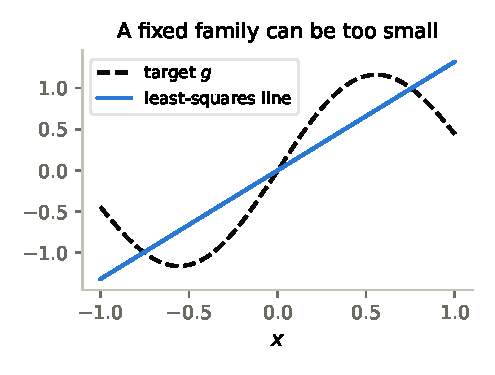
\includegraphics[width=\textwidth]{linear_fit.pdf}
\end{column}
\end{columns}
\nbref{10}
\end{frame}


% =========================================================================
\section{Universal approximation}

\begin{frame}{Two histories}
\footnotesize
\alert{Approximation:} which building blocks can describe every continuous function?
\begin{center}
\resizebox{\textwidth}{!}{%
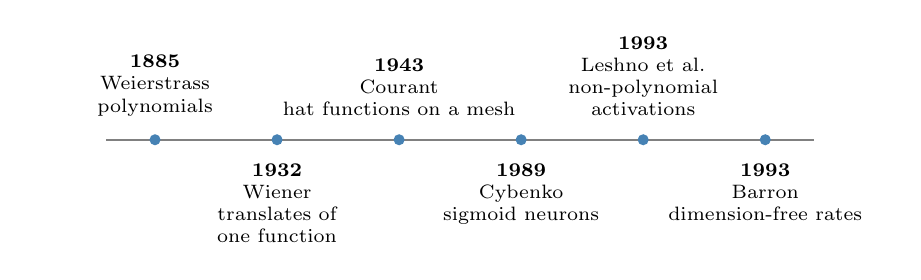
\begin{tikzpicture}[x=1.55cm, every node/.style={font=\scriptsize}]
  \draw[gray, line width=0.8pt] (-0.4,0) -- (5.4,0);
  \foreach \x/\yr/\txt/\anc/\dy in {
     0/1885/{Weierstrass\\polynomials}/south/0.18,
     1/1932/{Wiener\\translates of one function}/north/-0.18,
     2/1943/{Courant\\hat functions on a mesh}/south/0.18,
     3/1989/{Cybenko\\sigmoid neurons}/north/-0.18,
     4/1993/{Leshno et al.\\non-polynomial activations}/south/0.18,
     5/1993/{Barron\\dimension-free rates}/north/-0.18}
  {
    \fill[boxframe] (\x,0) circle (2pt);
    \node[anchor=\anc, align=center, text width=3.0cm] at (\x,\dy) {\textbf{\yr}\\\txt};
  }
\end{tikzpicture}}
\end{center}

\alert{Optimization:} how are the parameters found?
\begin{center}
\resizebox{\textwidth}{!}{%
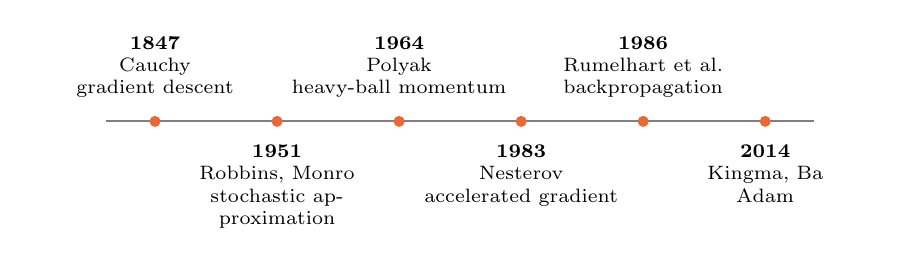
\begin{tikzpicture}[x=1.55cm, every node/.style={font=\scriptsize}]
  \draw[gray, line width=0.8pt] (-0.4,0) -- (5.4,0);
  \foreach \x/\yr/\txt/\anc/\dy in {
     0/1847/{Cauchy\\gradient descent}/south/0.18,
     1/1951/{Robbins, Monro\\stochastic approximation}/north/-0.18,
     2/1964/{Polyak\\heavy-ball momentum}/south/0.18,
     3/1983/{Nesterov\\accelerated gradient}/north/-0.18,
     4/1986/{Rumelhart et al.\\backpropagation}/south/0.18,
     5/2014/{Kingma, Ba\\Adam}/north/-0.18}
  {
    \fill[ctrl] (\x,0) circle (2pt);
    \node[anchor=\anc, align=center, text width=3.0cm] at (\x,\dy) {\textbf{\yr}\\\txt};
  }
\end{tikzpicture}}
\end{center}
\end{frame}


% =========================================================================
\begin{frame}{One recipe, four families}
An \alert{ansatz} is a choice of model family. A common recipe adds simple pieces: $f(x)=\sum_{j=1}^{m}c_j\,\varphi_j(x)$.

\medskip
\footnotesize
\renewcommand{\arraystretch}{1.55}
\begin{tabularx}{\textwidth}{@{}>{\raggedright\arraybackslash}X l l@{}}
\toprule
\textbf{Idea} & \textbf{Building block $\varphi_j(x)$} & \textbf{Model $f(x)$} \\
\midrule
1885, Weierstrass \citep{weierstrass1885}: polynomials & $x^{j}$ & $\sum_{j=0}^{m-1}c_j\,x^{j}$ \\
1932, Wiener \citep{wiener1932}: translates of one function & $\varphi(x-t_j)$,\ \ $\varphi(x)=e^{-x^2/(2h^2)}$ & $\sum_{j=1}^{m}c_j\,\varphi(x-t_j)$ \\
1943, Courant \citep{courant1943}: simple functions on mesh cells & $\max\big(0,\,1-|x-x_j|/h\big)$ & $\sum_{j=1}^{m}c_j\,\varphi_j(x)$ \\
1989, Cybenko \citep{cybenko1989}: neurons in one hidden layer & $\sigma(a_jx+b_j)$,\ \ $\sigma(t)=\frac{1}{1+e^{-t}}$ & $c_0+\sum_{j=1}^{m-1}c_j\,\sigma(a_jx+b_j)$ \\
\bottomrule
\end{tabularx}
\nbref{10 \S1}
\end{frame}


% =========================================================================
\begin{frame}{Four families, one target}
\begin{center}
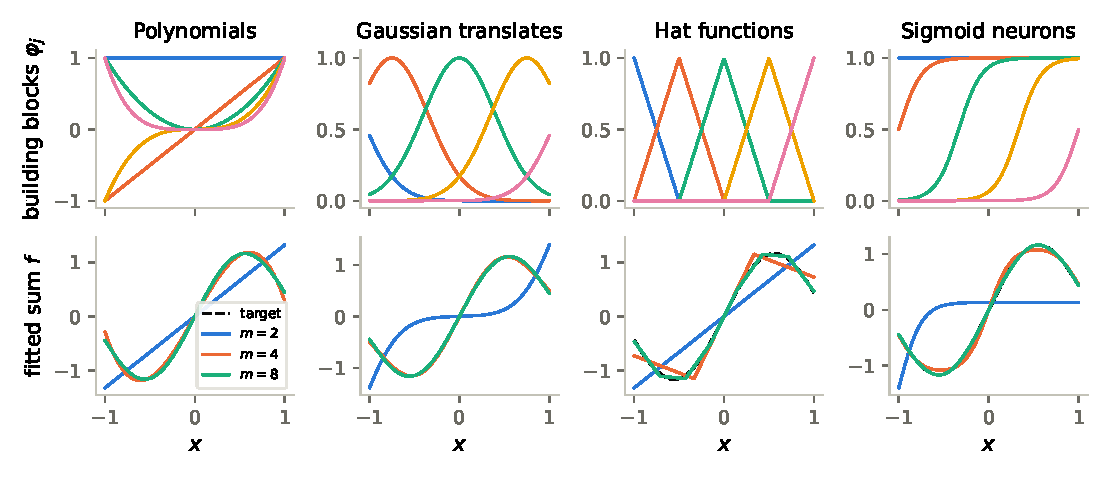
\includegraphics[width=\textwidth]{families.pdf}
\end{center}
\footnotesize
\alert{Top:} five building blocks of each family. \alert{Bottom:} the least-squares fit of $g$ with $m=2,4,8$ pieces.

With eight pieces, three of the four fits can no longer be told apart from the target; the hat functions still show their corners.
\nbref{10 \S2}
\end{frame}


% =========================================================================
\begin{frame}{Density: what the theorems say}
\small
\begin{mathbox}{Definition (density)}
A family $\mathcal F$ of functions is \textbf{dense} in $C([-1,1])$ if for every continuous $g$ and every $\varepsilon>0$ there is $f\in\mathcal F$ with $\max_{x\in[-1,1]}|g(x)-f(x)|<\varepsilon$.
\end{mathbox}
\begin{mathbox}{Theorem (Cybenko, 1989)}
Let $\sigma$ be continuous with $\sigma(t)\to0$ as $t\to-\infty$ and $\sigma(t)\to1$ as $t\to+\infty$. Then the sums $\sum_{j=1}^{m}c_j\,\sigma(a_j\cdot x+b_j)$, with $a_j\in\R^d$ and $b_j,c_j\in\R$, are dense in $C([0,1]^d)$ \citep{cybenko1989}.
\end{mathbox}
\footnotesize
\begin{itemize}
\item Density holds for every continuous activation that \alert{is not a polynomial} \citep{leshno1993}: the ReLU is covered.
\item Wiener's theorem is about $L^1(\R)$: the translates of $\varphi$ span a dense subspace if and only if $\hat\varphi$ has no zeros \citep{wiener1932}.
\item \alert{Existence is the starting point.} Density says neither how many pieces are needed nor how to find them.
\end{itemize}
\end{frame}


% =========================================================================
\begin{frame}{Why sigmoids are dense: a construction in one dimension}
\begin{center}
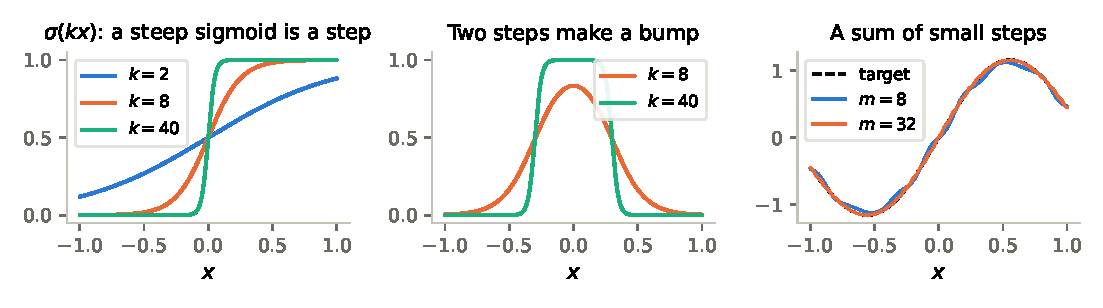
\includegraphics[width=0.9\textwidth]{sigmoid_construction.pdf}
\end{center}
\footnotesize
One neuron per cell of a mesh with nodes $s_0<\dots<s_m$, spacing $h$ and midpoints $t_j$:
\[
f_m(x)=g(s_0)+\sum_{j=1}^{m}\big(g(s_j)-g(s_{j-1})\big)\,\sigma\big(k\,(x-t_j)\big),\qquad k=6/h.
\]
\begin{itemize}
\item Each neuron is nearly a step at $t_j$, and the outer weights are the increments of $g$: a staircase that follows $g$.
\item $g$ is \emph{uniformly} continuous, so the increments are small when $h$ is small: $f_m\to g$ uniformly.
\item The error is $0.085$ for $m=8$ and $0.017$ for $m=32$, only about $1/m$. \alert{Density holds, but this is far from the best use of $m$ neurons.}
\end{itemize}
\end{frame}


% =========================================================================
\begin{frame}{Density by duality: Cybenko's proof and Kalman's}
\footnotesize
\begin{columns}[T,onlytextwidth]
\begin{column}{0.485\textwidth}
\alert{\textbf{Cybenko: density}}

\smallskip
Suppose the neurons $\sigma(a\cdot x+b)$ do \emph{not} span a dense subspace of $C(K)$, $K=[0,1]^d$.
\begin{enumerate}
\item Hahn--Banach, Riesz: there is a measure $\mu\neq0$ on $K$ with
$\int_K\sigma(a\cdot x+b)\,d\mu=0$ for all $a,b$.
\item Let the neuron become a step: $\mu$ vanishes on every half-space.
\item Hence $\hat\mu=0$ and $\mu=0$: a contradiction.
\end{enumerate}
\end{column}
\begin{column}{0.485\textwidth}
\alert{\textbf{Kalman: controllability (lecture 01)}}

\smallskip
Suppose the reachable directions $\Range L_T$ are \emph{not} all of $\R^n$.
\begin{enumerate}
\item There is $v\neq0$ with
$\int_0^T\langle B^*e^{A^*(T-s)}v,u(s)\rangle\,ds=0$ for all $u$.
\item Choose $u$ well: $B^*e^{A^*(T-s)}v=0$ on $[0,T]$.
\item Hence $v\perp A^jB$ for all $j$; by the rank condition, $v=0$: a contradiction.
\end{enumerate}
\end{column}
\end{columns}

\medskip
\begin{mathbox}{The common pattern}
What we can produce is dense (or everything) if and only if \emph{nothing nonzero is orthogonal to it}: a \alert{uniqueness} property of a dual object. For the heat equation, approximate controllability is the unique continuation of the adjoint (notebook 07).
\end{mathbox}
\scriptsize Cybenko's paper appeared in \emph{Mathematics of Control, Signals, and Systems}.
\end{frame}


% =========================================================================
\begin{frame}{From approximation to optimization}
\small
\alert{Fixed pieces: a linear problem.} With $\Phi_{ij}=\varphi_j(x_i)$, least squares has an explicit solution:
\[
\min_{c\in\R^m}\|\Phi c-y\|^2\qquad\Longleftrightarrow\qquad\Phi^\top\Phi\,c=\Phi^\top y .
\]
\alert{A network also moves and reshapes its pieces.} In
\[
f(x;w)=c_0+\sum_{j}c_j\,\sigma(a_jx+b_j),\qquad w=(a,b,c),
\]
the inner parameters $(a_j,b_j)$ enter through $\sigma$, and the training loss
\[
F(w)=\frac1N\sum_{i=1}^N\big(f(x_i;w)-y_i\big)^2
\]
is in general \alert{not convex}.

\begin{center}
\emph{Approximation asks whether good parameters exist. Optimization tries to find them.}
\end{center}
\nbref{10 \S2}
\end{frame}


% =========================================================================
\section{Gradient descent}

\begin{frame}{Gradient descent: direction and step size}
\small
Let $F$ be differentiable; we want $\min_{w\in\R^d}F(w)$. Near $w_k$, Taylor's formula gives a \emph{linear} model:
\[
F(w)=F(w_k)+\langle\nabla F(w_k),\,w-w_k\rangle+o(\|w-w_k\|).
\]
If $\nabla F(w_k)\neq0$ this model is unbounded below. Add a quadratic penalty for long steps:
\begin{mathbox}{Gradient descent}
\[
\begin{aligned}
w_{k+1}&=\argmin_{u\in\R^d}\Big\{F(w_k)+\langle\nabla F(w_k),\,u-w_k\rangle+\tfrac1{2\eta}\|u-w_k\|^2\Big\}\\
&=w_k-\eta\,\nabla F(w_k).
\end{aligned}
\]
\end{mathbox}
\begin{itemize}
\item The gradient picks the \alert{direction}; the \alert{learning rate} $\eta>0$ picks how far.
\item It is the explicit Euler scheme, with time step $\eta$, for the \alert{gradient flow} $\dot w=-\nabla F(w)$.
\end{itemize}
\nbref{10 \S3}
\end{frame}


% =========================================================================
\begin{frame}{The step size on a quadratic}
\begin{center}
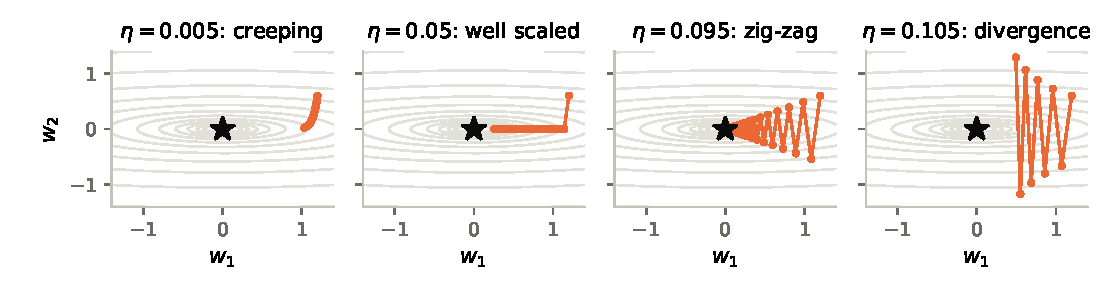
\includegraphics[width=\textwidth]{gd_step_sizes.pdf}
\end{center}
\footnotesize
For $F(w)=\tfrac12\big(w_1^2+20\,w_2^2\big)$ each step multiplies the two coordinates by fixed factors:
\[
w_1\ \mapsto\ (1-\eta)\,w_1,\qquad\qquad w_2\ \mapsto\ (1-20\,\eta)\,w_2 .
\]
\begin{itemize}
\item \alert{Stability.} The iteration converges if and only if $|1-20\eta|<1$, that is, $\eta<2/L$ with $L=20$ the largest curvature. At $\eta=0.105$ the factor is $-1.1$: divergence.
\item \alert{Speed.} The flat direction contracts by $1-\eta\ge1-2/L$ at best. The ratio of the curvatures, the \alert{condition number} $\kappa=20$, limits the speed of every stable step size.
\end{itemize}
\nbref{10 \S3}
\end{frame}


% =========================================================================
\begin{frame}{Smoothness and the descent lemma}
\small
\begin{mathbox}{Assumption ($L$-smoothness)}
$F$ is differentiable and $\nabla F$ is $L$-Lipschitz: $\|\nabla F(u)-\nabla F(v)\|\le L\,\|u-v\|$ for all $u,v$.
\end{mathbox}
\footnotesize
If $F$ is twice differentiable this means $-L\,I\preceq\nabla^2F(w)\preceq L\,I$: the curvature is bounded. \alert{Nothing forces $F$ to be convex.}
\small
\begin{mathbox}{Lemma (descent lemma)}
\[
F(v)\le F(u)+\langle\nabla F(u),\,v-u\rangle+\frac L2\,\|v-u\|^2\qquad\text{for all }u,v.
\]
\end{mathbox}
\footnotesize
\emph{Proof.} By the fundamental theorem of calculus along the segment $u+t(v-u)$,
\[
F(v)-F(u)-\langle\nabla F(u),v-u\rangle=\int_0^1\big\langle\nabla F\big(u+t(v-u)\big)-\nabla F(u),\ v-u\big\rangle\,dt .
\]
By Cauchy--Schwarz and the Lipschitz assumption, the integrand is at most $L\,t\,\|v-u\|^2$, and $\int_0^1L\,t\,dt=L/2$. \hfill$\square$
\nbref{10 \S4}
\end{frame}


% =========================================================================
\begin{frame}{Gradient descent minimizes an upper bound}
\begin{columns}[T]
\begin{column}{0.42\textwidth}
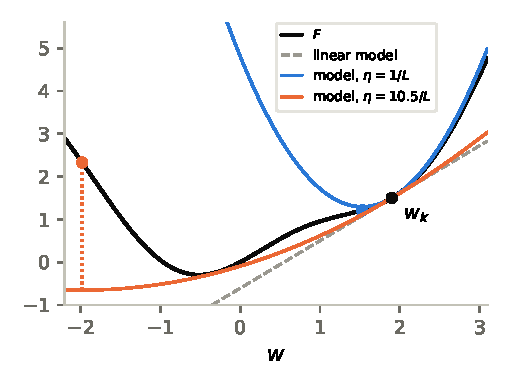
\includegraphics[width=\textwidth]{descent_lemma.pdf}

\scriptsize $F(w)=\tfrac12w^2+\tfrac12\sin(2w)$, with $L=3$. The dots are the next iterates $w_{k+1}$ for two step sizes.
\end{column}
\begin{column}{0.58\textwidth}
\footnotesize
Take $u=w_k$ in the lemma. If $1/\eta\ge L$, the model that defined gradient descent,
\[
m_k(v)=F(w_k)+\langle\nabla F(w_k),v-w_k\rangle+\tfrac1{2\eta}\|v-w_k\|^2,
\]
is a \alert{global upper bound} of $F$ that touches $F$ at $w_k$. Minimizing it cannot increase $F$:
\[
F(w_{k+1})\le m_k(w_{k+1})=F(w_k)-\frac\eta2\,\|\nabla F(w_k)\|^2 .
\]
For any $\eta$, the lemma with $v=w_{k+1}$ gives
\[
F(w_{k+1})\le F(w_k)-\eta\Big(1-\frac{L\eta}2\Big)\|\nabla F(w_k)\|^2 ,
\]
a guaranteed decrease exactly when $\eta<2/L$: the threshold seen on the quadratic.

\smallskip
With a much larger step (orange) the model is not an upper bound: it promises a decrease, and $F$ increases.
\end{column}
\end{columns}
\end{frame}


% =========================================================================
\begin{frame}{Theorem 1: the gradient becomes small}
\small
\begin{mathbox}{Theorem 1 (decay of the gradient)}
Let $F$ be $L$-smooth and bounded below by $F^\star$, and let $0<\eta\le1/L$. Then gradient descent satisfies
\[
F(w_{k+1})\le F(w_k)-\frac\eta2\,\|\nabla F(w_k)\|^2,
\quad
\min_{0\le k<K}\|\nabla F(w_k)\|^2\le\frac{2\big(F(w_0)-F^\star\big)}{\eta\,K}.
\]
\end{mathbox}
\emph{Proof.} The first inequality is the previous slide, since $\eta L\le1$ gives $1-L\eta/2\ge1/2$. Summing it for $k=0,\dots,K-1$, the values of $F$ telescope:
\[
\frac\eta2\sum_{k=0}^{K-1}\|\nabla F(w_k)\|^2\le F(w_0)-F(w_K)\le F(w_0)-F^\star,
\]
and the minimum of $K$ terms is at most their average. \hfill$\square$

\medskip
\footnotesize
$F$ decreases along the iteration: it is a \alert{Lyapunov function}. No convexity is used, and the conclusion is weak: a small gradient can be a local minimum or a saddle point.
\nbref{10 \S4}
\end{frame}


% =========================================================================
\begin{frame}{Theorem 2: the convex case}
\small
\begin{mathbox}{Theorem 2 (convex case)}
If in addition $F$ is convex with a minimizer $w^\star$, and $0<\eta\le1/L$, then
\[
F(w_K)-F^\star\le\frac{\|w_0-w^\star\|^2}{2\,\eta\,K}.
\]
\end{mathbox}
\footnotesize
\emph{Proof.} Expand the distance to $w^\star$ and use convexity, $\langle\nabla F(w_k),w_k-w^\star\rangle\ge F(w_k)-F^\star$:
\[
\|w_{k+1}-w^\star\|^2\le\|w_k-w^\star\|^2-2\eta\big(F(w_k)-F^\star\big)+\eta^2\|\nabla F(w_k)\|^2 .
\]
Theorem 1 bounds the last term by the decrease achieved, $\eta^2\|\nabla F(w_k)\|^2\le2\eta\big(F(w_k)-F(w_{k+1})\big)$, so
\[
\|w_{k+1}-w^\star\|^2\le\|w_k-w^\star\|^2-2\eta\big(F(w_{k+1})-F^\star\big).
\]
Sum over $k<K$. The left side telescopes, and $F(w_k)$ is non-increasing, so each of the $K$ terms on the right is at least $F(w_K)-F^\star$:
\[
2\,\eta\,K\,\big(F(w_K)-F^\star\big)\le\|w_0-w^\star\|^2-\|w_K-w^\star\|^2\le\|w_0-w^\star\|^2. \qquad\square
\]
\nbref{10 \S4}
\end{frame}


% =========================================================================
\begin{frame}{Three rates}
\footnotesize
\renewcommand{\arraystretch}{1.6}
\begin{tabularx}{\textwidth}{@{}>{\raggedright\arraybackslash}p{0.22\textwidth} >{\raggedright\arraybackslash}X >{\raggedright\arraybackslash}p{0.19\textwidth}@{}}
\toprule
\textbf{Assumptions on $F$} & \textbf{Guarantee for $0<\eta\le1/L$} & \textbf{Steps for tolerance $\varepsilon$} \\
\midrule
$L$-smooth, bounded below & $\min_{k<K}\|\nabla F(w_k)\|^2\le\dfrac{2\big(F(w_0)-F^\star\big)}{\eta K}$ & $O(\varepsilon^{-2})$ for $\|\nabla F\|\le\varepsilon$ \\
$L$-smooth, convex, with a minimizer & $F(w_K)-F^\star\le\dfrac{\|w_0-w^\star\|^2}{2\eta K}$ & $O(\varepsilon^{-1})$ \\
$L$-smooth, $\mu$-strongly convex & $F(w_K)-F^\star\le(1-\eta\mu)^K\big(F(w_0)-F^\star\big)$ & $O\big(\kappa\log\tfrac1\varepsilon\big)$,\ \ $\kappa=L/\mu$ \\
\bottomrule
\end{tabularx}

\medskip
\alert{The third row in one line.} Strong convexity gives $\|\nabla F(w)\|^2\ge2\mu\big(F(w)-F^\star\big)$. Insert it in Theorem 1: $F(w_{k+1})-F^\star\le(1-\eta\mu)\big(F(w_k)-F^\star\big)$.

\medskip
The \alert{condition number} $\kappa$ measures the difficulty of the problem for gradient descent \citep{nocedal2006}. In notebook 03 the same number, for the Gramian $\Gram_T$, sets the speed at which the minimal-norm control is computed.
\end{frame}


% =========================================================================
\section{Momentum}

\begin{frame}{Momentum: carry the previous step}
\footnotesize
In a narrow valley gradient descent zig-zags across the steep sides and creeps along the floor. Polyak's \alert{heavy-ball method} \citep{polyak1964} gives the iterate a velocity:
\[
v_{k+1}=\beta\,v_k-\eta\,\nabla F(w_k),\qquad w_{k+1}=w_k+v_{k+1},\qquad\beta\in[0,1).
\]
$\beta$ is the fraction of the previous step that is kept; $\beta=0$ is gradient descent.
\begin{center}
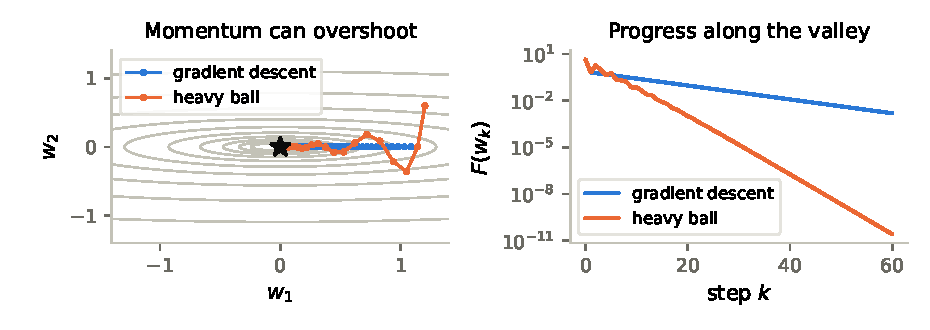
\includegraphics[width=0.74\textwidth]{momentum.pdf}
\end{center}
\scriptsize The quadratic of the previous slides, $\eta=0.05$, $\beta=0.6$. After 60 steps: $F=1.5\cdot10^{-3}$ for gradient descent, $2.6\cdot10^{-11}$ for the heavy ball.

\smallskip
\footnotesize
\alert{Two continuous-time limits.} Gradient descent follows $\dot w=-\nabla F(w)$. The heavy ball, with $\beta=1-a\sqrt\eta$ and time $\sqrt\eta$ per step, follows $\ddot w+a\,\dot w+\nabla F(w)=0$: a ball rolling on the loss surface with friction $a$, the \alert{damped oscillator} of lecture 01. Too little friction oscillates, too much creeps.
\nbref{10 \S5, 11 \S3}
\end{frame}


% =========================================================================
\begin{frame}{The same optimizers on three problems}
\begin{center}
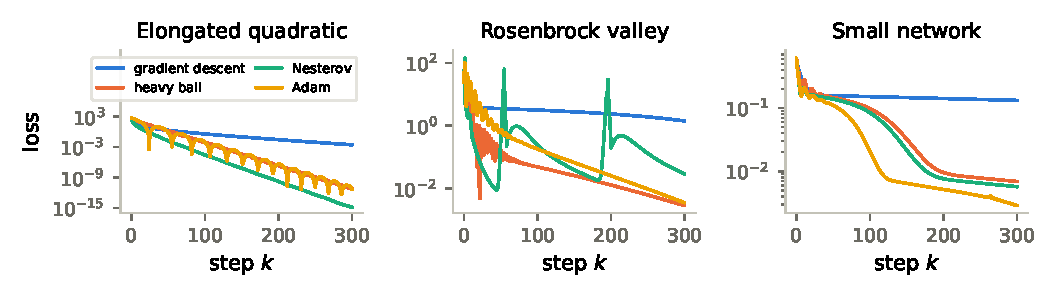
\includegraphics[width=0.93\textwidth]{optimizers.pdf}
\end{center}
\footnotesize
\begin{itemize}
\item \alert{Nesterov momentum} evaluates the gradient at a look-ahead point \citep{nesterov1983}.
\item \alert{RMSProp} and \alert{Adam} keep running averages of the gradients and of their squares, and scale the step coordinate by coordinate \citep{hinton2012,kingma2015}.
\end{itemize}
A quadratic with curvatures from $1$ to $100$, the curved Rosenbrock valley, and a network with $49$ parameters fitting $g$; 300 full-gradient steps from the same starting point.

\smallskip
A method that works well in a straight valley can behave differently when the valley bends. The learning rate of Adam is chosen separately: the curves illustrate behaviour, they do not rank the optimizers.
\nbref{10 \S5.1, 11}
\end{frame}


% =========================================================================
\section{Noise and mini-batches}

\begin{frame}{Non-convex problems: noise can leave a basin}
\footnotesize
Theorem 1 only promises a small gradient: gradient descent stays in its basin. Add white noise to the gradient flow, and discretize:
\[
dw_t=-\nabla F(w_t)\,dt+\sigma\,dB_t,\qquad
w_{k+1}=w_k-\eta\,\nabla F(w_k)+\sigma\sqrt\eta\,\xi_k,\quad \xi_k\sim\mathcal N(0,I).
\]
\begin{center}
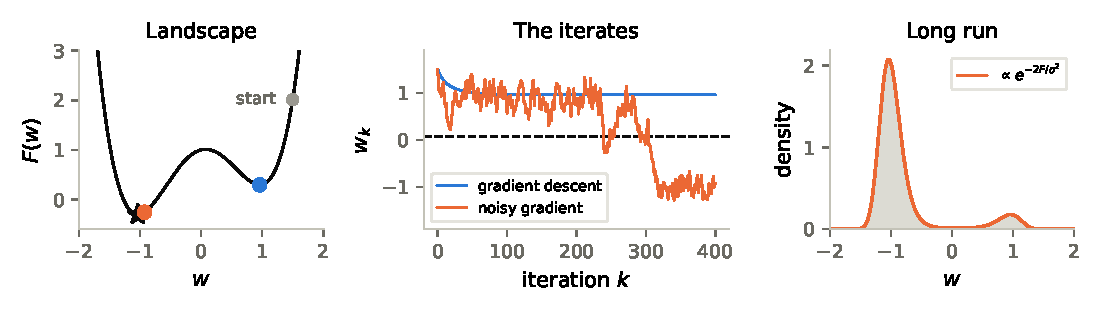
\includegraphics[width=0.84\textwidth]{double_well.pdf}
\end{center}
\begin{itemize}
\item $F(w)=(w^2-1)^2+0.3\,w$, from $w_0=1.5$. Gradient descent settles in the shallow well; with $\sigma=0.7$ the iterate crosses the barrier (dashed) at step 239.
\item In the long run the noisy iterates sample the \alert{Gibbs measure} $\propto e^{-2F/\sigma^2}$: 91\% of the time in the deep well.
\item A small $\sigma$ concentrates it on the global minimum \citep{geman1986}, but crossing a barrier $\Delta F$ takes a time of order $e^{2\Delta F/\sigma^2}$: \alert{accuracy against exploration}.
\end{itemize}
\nbref{10 \S6, 11 App.~A}
\end{frame}


% =========================================================================
\begin{frame}{Mini-batch gradients}
\footnotesize
The loss averages over $N$ samples; a \alert{mini-batch} $B_k$ uses a few of them:
\[
g_k=\frac1{|B_k|}\sum_{i\in B_k}\nabla_w\big(f(x_i;w_k)-y_i\big)^2,\qquad w_{k+1}=w_k-\eta\,g_k .
\]
\begin{itemize}
\item $g_k$ is an \alert{unbiased} estimate of $\nabla F(w_k)$ at a fraction $|B_k|/N$ of the cost. An \alert{epoch} is one pass through the data.
\item The randomness enters multiplied by $\eta$, not by $\sigma\sqrt\eta$: a different algorithm from the previous slide, with the same flavour.
\end{itemize}
\begin{center}
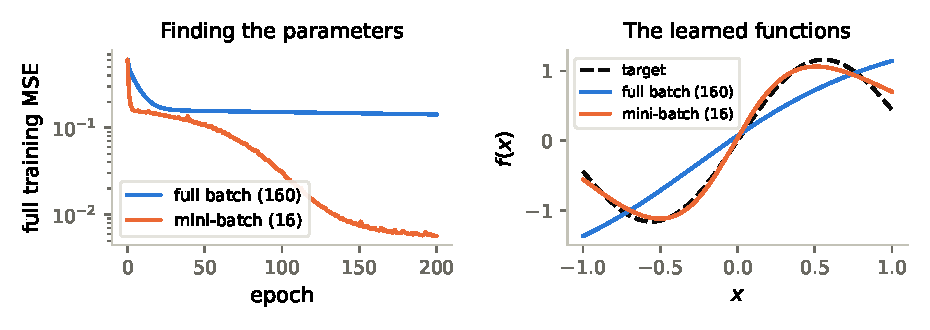
\includegraphics[width=0.68\textwidth]{minibatch.pdf}
\end{center}
\scriptsize A $\tanh$ network $1\to16\to1$ (49 parameters) on 160 samples of $g$, $\eta=0.05$, same initial weights, 200 epochs: training error $0.14$ with the full batch (200 steps) and $0.0057$ with batches of 16 (2000 steps).
\nbref{10 \S7}
\end{frame}


% =========================================================================
\section{Everything at once}

\begin{frame}{Everything at once: handwritten digits}
\begin{columns}[T]
\begin{column}{0.57\textwidth}
\footnotesize
\alert{Data.} MNIST \citep{lecun1998}: $60\,000$ training and $10\,000$ test images of $28\times28$ grey pixels. An input is $x\in\R^{784}$, its label a class $y\in\{0,\dots,9\}$.

\medskip
\alert{Model.} Two hidden layers of 16 neurons, ten outputs:
\[
f(x;w)=W_3\,\sigma\big(W_2\,\sigma(W_1x+b_1)+b_2\big)+b_3\in\R^{10},
\]
with $\sigma(t)=\max(0,t)$. Each hidden neuron computes $\sigma(a\cdot x+b)$: Cybenko's building block with a vector input. Altogether $13\,002$ parameters.

\medskip
\alert{Loss.} The softmax turns the ten outputs into probabilities, and the \alert{cross-entropy} is the negative log-probability of the correct class:
\[
p_j=\frac{e^{f_j}}{\sum_{l}e^{f_l}},\qquad
F(w)=-\frac1N\sum_{i=1}^N\log p_{y_i}(x_i;w).
\]
\end{column}
\begin{column}{0.43\textwidth}
\centering
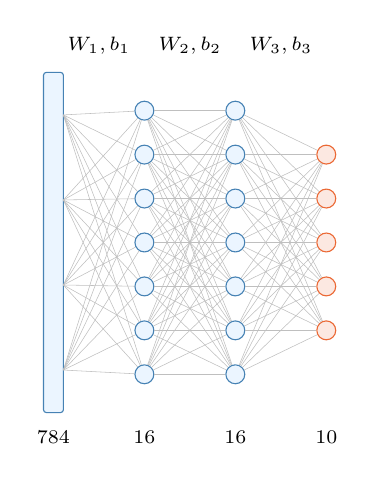
\begin{tikzpicture}[x=1.05cm, y=0.36cm, >=Stealth, font=\scriptsize]
  % 784 inputs drawn as a tall bar, 16 + 16 hidden neurons and 10 outputs (a few of each drawn)
  \draw[fill=boxbg, draw=boxframe, rounded corners=1pt] (-0.12,-6) rectangle (0.12,6);
  \foreach \i in {1,...,7} {
    \node[circle, draw=boxframe, fill=boxbg, inner sep=0pt, minimum size=2.4mm] (h1\i) at (1.1,{(4-\i)*1.55}) {};
    \node[circle, draw=boxframe, fill=boxbg, inner sep=0pt, minimum size=2.4mm] (h2\i) at (2.2,{(4-\i)*1.55}) {};
  }
  \foreach \i in {1,...,5}
    \node[circle, draw=ctrl, fill=ctrl!15, inner sep=0pt, minimum size=2.4mm] (o\i) at (3.3,{(3-\i)*1.55}) {};
  \foreach \i in {1,...,7} {
    \foreach \y in {-4.5,-1.5,1.5,4.5} \draw[black!25, line width=0.2pt] (0.12,\y) -- (h1\i);
    \foreach \j in {1,...,7} \draw[black!25, line width=0.2pt] (h1\i) -- (h2\j);
    \foreach \j in {1,...,5} \draw[black!25, line width=0.2pt] (h2\i) -- (o\j);
  }
  \node[below] at (0,-6.3) {$784$};
  \node[below] at (1.1,-6.3) {$16$};
  \node[below] at (2.2,-6.3) {$16$};
  \node[below] at (3.3,-6.3) {$10$};
  \node[above] at (0.55,6.3) {$W_1,b_1$};
  \node[above] at (1.65,6.3) {$W_2,b_2$};
  \node[above] at (2.75,6.3) {$W_3,b_3$};
\end{tikzpicture}

\medskip
\scriptsize
$784\cdot16+16=12\,560$\\
$16\cdot16+16=272$\\
$16\cdot10+10=170$\\[2pt]
The network of 3Blue1Brown's \href{https://www.youtube.com/watch?v=aircAruvnKk}{\emph{But what is a neural network?}}
\end{column}
\end{columns}
\nbref{10 \S8}
\end{frame}


% =========================================================================
\begin{frame}[fragile]{Training the digit classifier}
\begin{lstlisting}
optimizer = torch.optim.Adam(net.parameters(), lr=1e-3)
for epoch in range(5):
    order = torch.randperm(60000)             # a new random order of the data
    for batch in order.split(64):             # 938 mini-batches per epoch
        optimizer.zero_grad()                 # clear old derivatives
        loss = cross_entropy(net(images[batch]), labels[batch])
        loss.backward()                       # backpropagation
        optimizer.step()                      # update the parameters
\end{lstlisting}
\begin{columns}[c]
\begin{column}{0.66\textwidth}
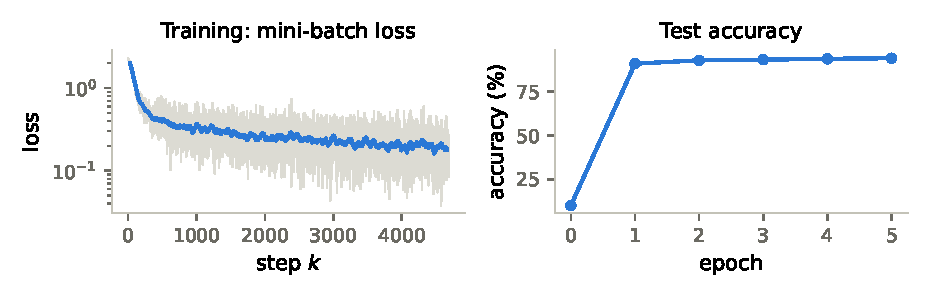
\includegraphics[width=\textwidth]{mnist_training.pdf}
\end{column}
\begin{column}{0.34\textwidth}
\footnotesize
Today in eight lines: neurons, a loss that is an average, mini-batches, adaptive steps with momentum (Adam).

\medskip
$4\,690$ steps: seconds on a laptop. Grey is the loss of each mini-batch, blue its moving average.

\medskip
Test accuracy, on images never used for training: \alert{94.0\%}.
\end{column}
\end{columns}
\nbref{10 \S8}
\end{frame}


% =========================================================================
\begin{frame}{What the trained network predicts}
\begin{center}
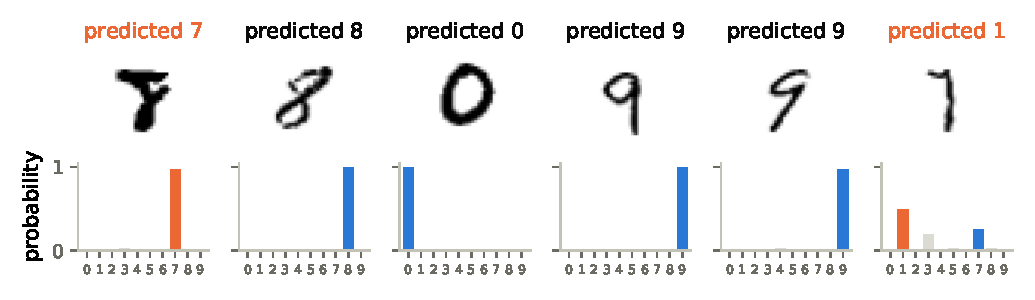
\includegraphics[width=0.88\textwidth]{mnist_predictions.pdf}
\end{center}
\footnotesize
Six test images drawn at random, with the probabilities $p_j(x;w)$: blue is the true class, orange a wrong prediction.
\begin{itemize}
\item Right and confident on four. Wrong on two: an 8 read as a 7 \alert{with high confidence}, and a 7 read as a 1 with hesitation. A softmax output need not be a calibrated probability.
\item This model ignores that the input is an image: shuffling the 784 pixels, in the same way for every image, only relabels the columns of $W_1$.
\item LeNet-5, a \emph{convolutional} network, reached about $99\%$ in 1998 \citep{lecun1998}. \alert{The architecture matters:} next lecture.
\end{itemize}
\nbref{10 \S8}
\end{frame}


% =========================================================================
\begin{frame}{Key takeaways}
\small
\begin{enumerate}
\item \alert{Representation.} Different building blocks describe the same target. Density is an existence statement: it gives neither the number of pieces nor their parameters. Its proof is a duality argument, as for controllability.
\item \alert{Gradient descent} minimizes a linear model plus a quadratic penalty for long steps. Smoothness controls the step size, $\eta<2/L$; convexity gives a bound on the objective gap; the condition number sets the speed.
\item \alert{Momentum} is a damped second-order dynamics. It accelerates along a valley, at the risk of overshooting.
\item \alert{Noise} trades accuracy for exploration. Brownian noise and mini-batch noise are different constructions with the same trade-off.
\item \alert{In practice} the pieces combine: a $784\to16\to16\to10$ network, the cross-entropy, mini-batches and Adam read handwritten digits with $94\%$ test accuracy.
\end{enumerate}

\medskip
\footnotesize
\alert{Next lecture}, \emph{The training loop}, takes the four choices behind the digit classifier in turn: the representation of the data, the architecture, the loss and the optimizer.
\end{frame}


% =========================================================================
\begin{frame}[allowframebreaks]{References}
\scriptsize
\bibliographystyle{plainnat}
\bibliography{universal_approximation_and_optimization}
\end{frame}

\end{document}
